%%%%%%%%%%%%%%%%%%%%%%%%%%%%POSTER%%%%%%%%%%%%%%%%%%%%%%%%%%%%%%
\begin{columns}
\column{1}
\block{Introdução}{
As balanças foram criadas por necessidade e são utilizadas para medir uma das grandezas fundamentais da física, a massa. A massa é uma das grandezas intrínsecas dos objetos, que se mede pela suas resistência à aceleração.
\\
\\
Determinar a massa dos objetos é uma ferramenta em que empurra o desenvolvimento comercial, industrial e científico. Existe uma constante evolução para adquirir equipamentos com maior precisão e imunes a interferências para medir esta grandeza beneficiando o desenvolvimento cientifico. Motivo deste projeto de criar uma balança digital recorrendo aos materiais disponíveis no mercado.
}
\end{columns}
\begin{columns}
\column{0.1}
\column{0.8}
\block{Kit Desenvolvimento}{
	\begin{tikzfigure}
		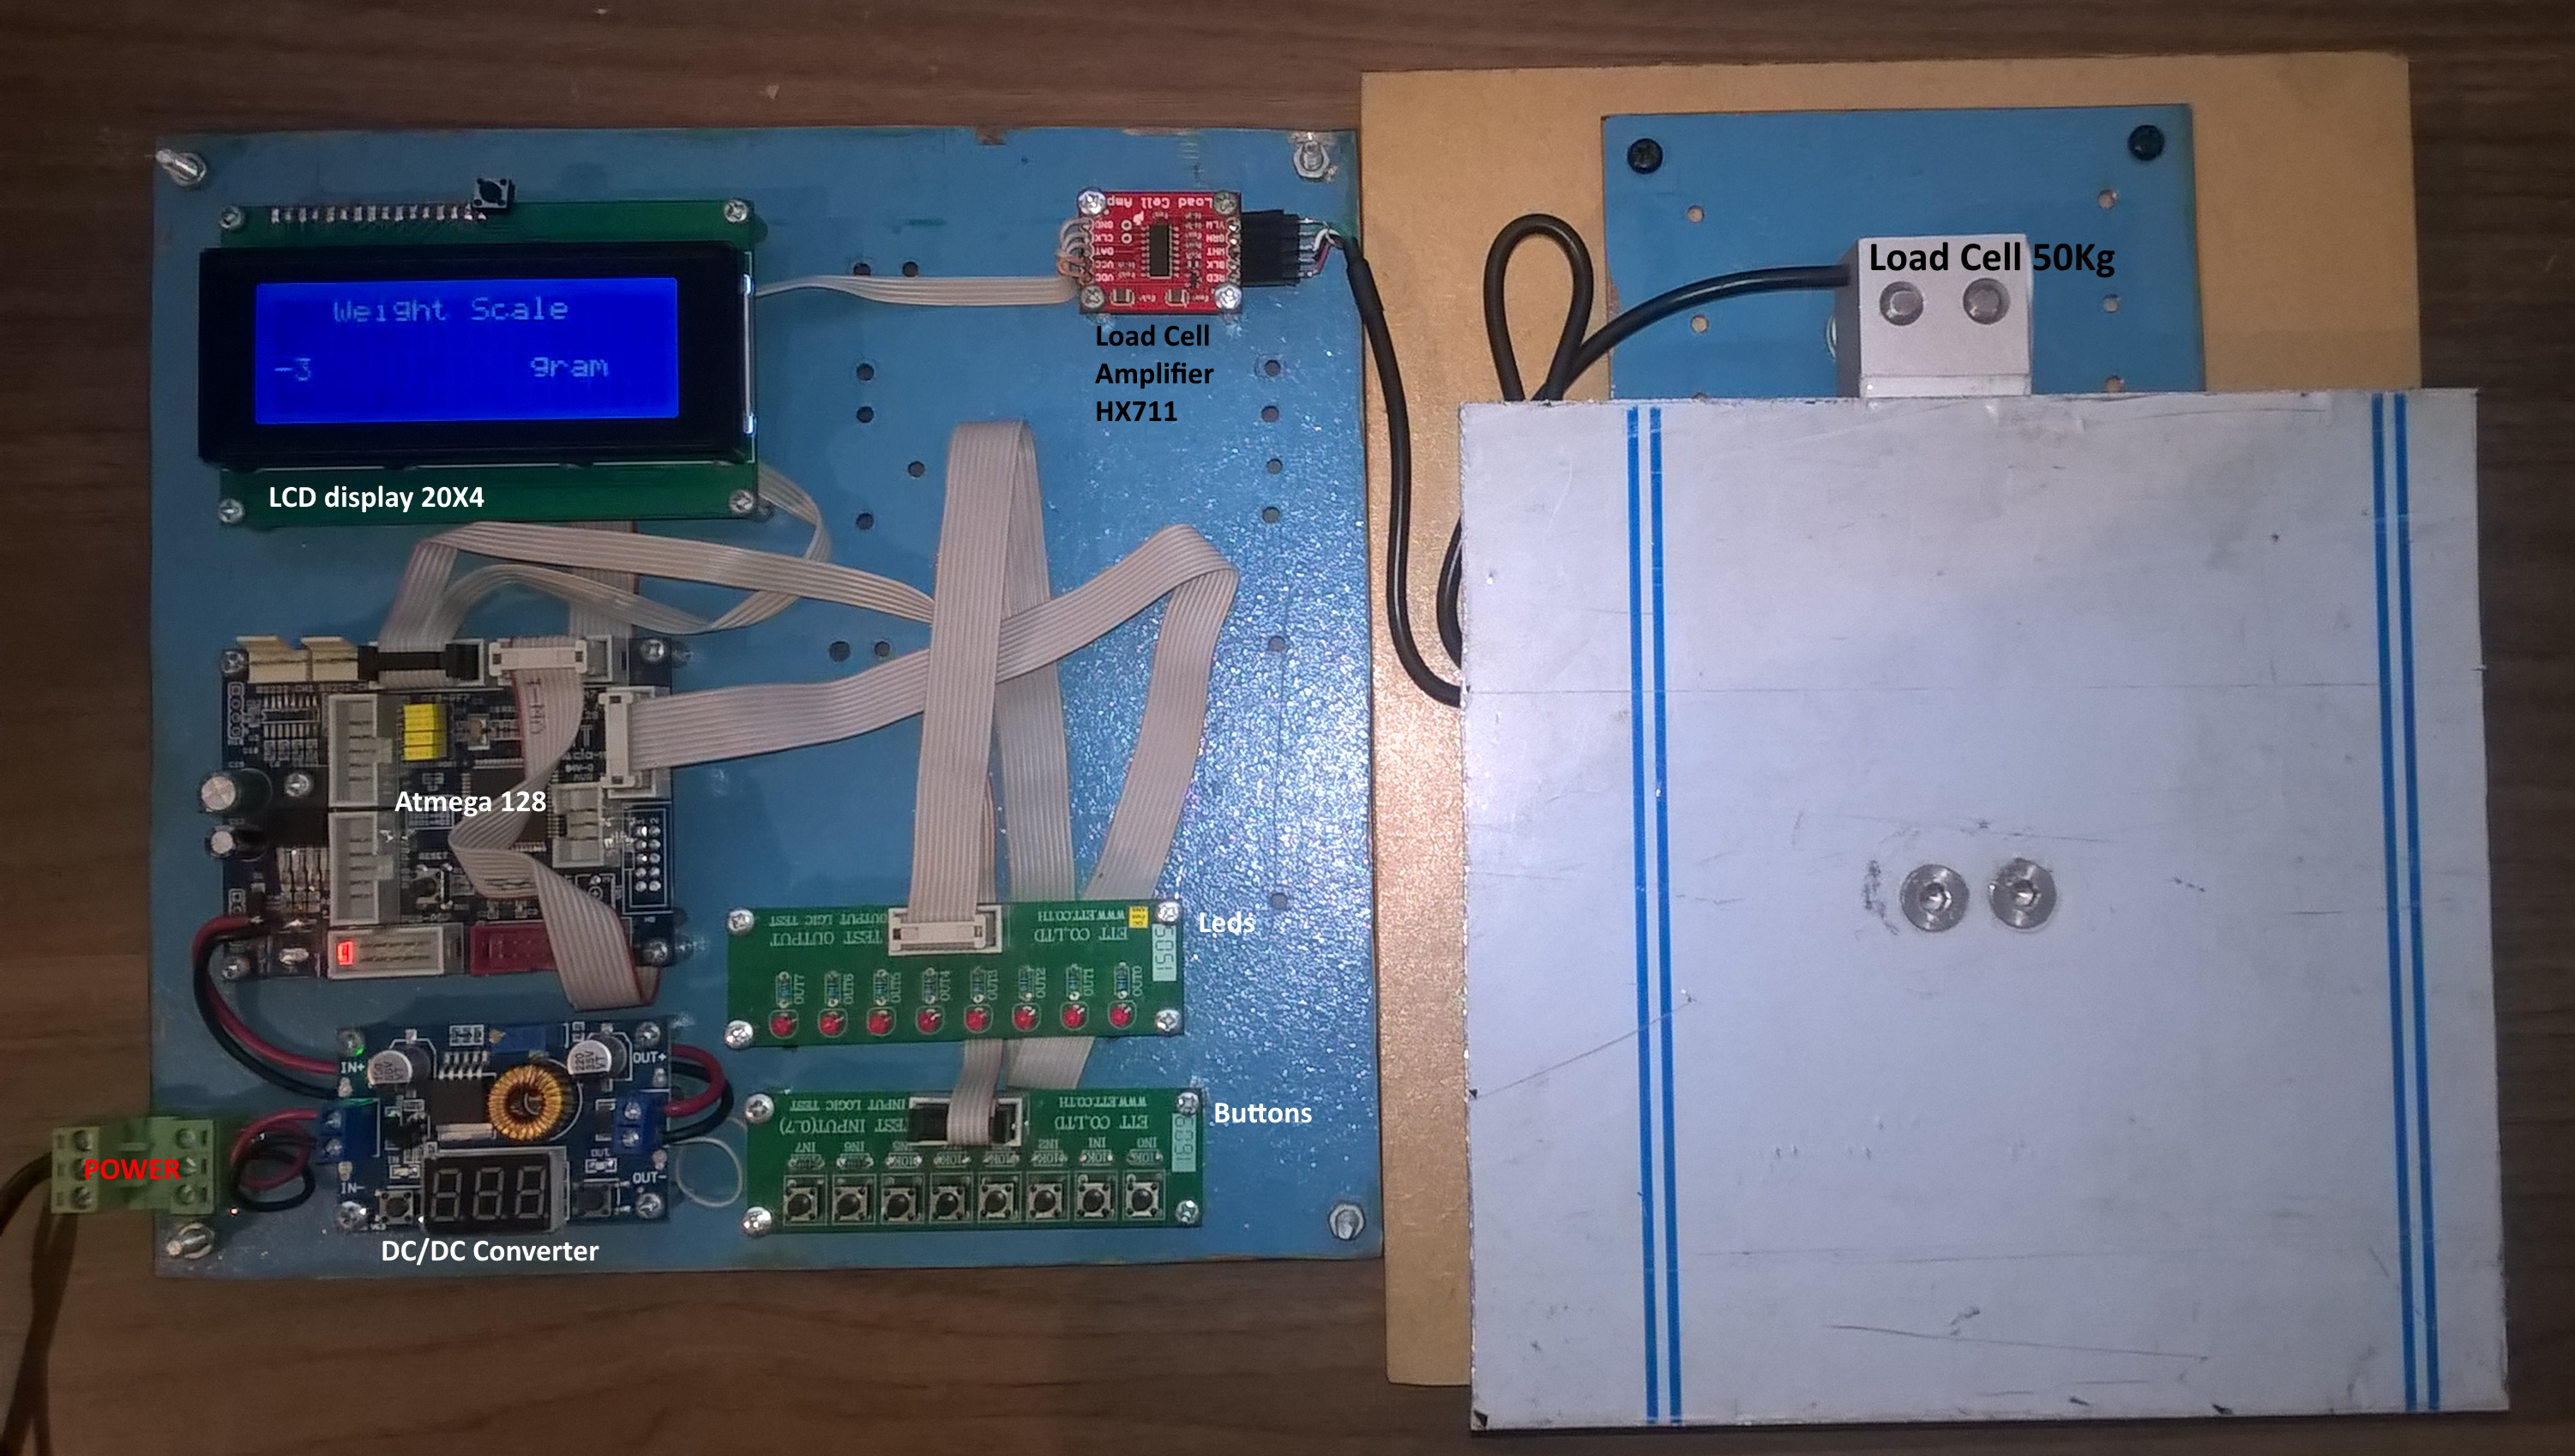
\includegraphics[width=0.7\textwidth]{./image/PESTA/kit/Kit_Desenvolvimento_2.jpg}
	\end{tikzfigure}
}
\end{columns}
\begin{columns}
\column{0.5}
\block{Sensor}{
O sensor é um transdutor utilizado para converter energia de uma natureza para outra e servir como entrada de um sistema de controlo, são os elementos principais de interface com o mundo real para o analógico.
\\
Neste projeto é o caso de utilizar uma célula de carga de tipo piezoresistivo para determinar a massa dos objetos.	
}
\column{0.5}
\block{Informação e Controlo}{
O tratamento da informação e sua comunicação nas várias etapas até chegar ao sistema digital têm grande complexidade. Requer muitos conhecimentos em diversas áreas.
\\
Usando a linguagem C e um microcontrolador foi possível desenvolver este projeto, com um controlo intuitivo e fácil de se replicar.
}
\end{columns}
\begin{columns}
\column{1}
\block{Conclusões}{
	\bigskip
	\coloredbox{
		\hspace{.2cm}
		\textbf{Importancia:}\\ \\
		\begin{minipage}[b!]{.37\linewidth}
			\begin{itemize}
				\item Acumolação de conhecimentos e documentação (\textbf{\textit{github}}).
				\item Utilização das ferramentas (multimetro, osciloscopio, \textbf{IDE}, etc).
				\item Leitura e interpretação de \textit{datasheets} e manuais.
			\end{itemize}
		\end{minipage}
		\begin{minipage}[b!]{.3\linewidth}
			\begin{itemize}
				\item Criar uma methologia de trabalho.
				\item Pesquisar de literatura.
				\item Dominar a linguagem \textbf{C}.
			\end{itemize}
		\end{minipage}
		\begin{minipage}[b!]{.4\linewidth}
			\begin{itemize}
				\item Criar drivers e livrarias independentes.
				\item Obter \textit{Know How} em diversas areas.
				\item Experimentar.
			\end{itemize}
		\end{minipage}
	}
	\bigskip
	\bigskip
	\coloredbox{
		\centering
		\textbf{Efeitos Observados:} \\
		\begin{minipage}[b!]{\linewidth}
			\hspace{3cm}
			\begin{minipage}[b!]{.2\linewidth}
			\begin{itemize}
				\item Ruído
				\item Temperatura
				\item Humidade
				\item \textit{Long term shift}
				\item Histerese
			\end{itemize}
			\end{minipage}
			\begin{minipage}[b!]{.6\linewidth}
				Ao executar este projecto teve de se ter em conta interferencia exteriores, tais como colocar o amplificador de sinal o mais próximo do sensor e afastado do ruído do circuito electrónico. Foi observado os efeito a longo prazo das leituras e seu desvio.
				\vspace{1cm}
			\end{minipage}
		\end{minipage}
	}
	\vspace{5cm}
}
\note[targetoffsetx=-34cm, targetoffsety=-8.5cm, width=.3\linewidth]{\bigskip
	\texttt{https://github.com/sergio1020881/PESTA2021}
}
%
\includegraphics[width=.8\textwidth]{./image/Capa/Footer_1.png}
\end{columns}
%%%%%%%%%%%%%%%%%%%%%%%%%%%%%%%%%%%%%%%%%%%%%%%%%%%%%%%%%%%%%%%%
